%----------------------------------------------------------------------------------------
%
% A LaTeX-template for 1DV510. Modified and translated by Björn Lindenberg at LNU.
% Based on an original master thesis template created by Marcus Wilhelmsson at LNU.
%
%----------------------------------------------------------------------------------------

% Settings and document configuration

\documentclass[a4paper,12pt]{article} 
\usepackage[T1]{fontenc} 
\usepackage{times} 
\usepackage[swedish,english]{babel} 
\usepackage[utf8]{inputenc} 
\usepackage{dtk-logos} 
\usepackage{wallpaper} 
\usepackage[absolute]{textpos} 
\usepackage[top=2cm, bottom=2.5cm, left=3cm, right=3cm]{geometry} 
\usepackage[parfill]{parskip} 
\usepackage{csquotes} 
\usepackage{float} 
\usepackage{lipsum} % Used for dummy text. Can be removed.
\usepackage{listings, color}

\lstdefinestyle{Asm}{
  belowcaptionskip=1\baselineskip,
  breaklines=true,
  frame=L,
  xleftmargin=\parindent,
  language=[x86masm]Assembler,
  showstringspaces=false,
  basicstyle=\footnotesize\ttfamily,
  keywordstyle=\bfseries\color{purple!40!black},
  commentstyle=\itshape\color{green!40!black},
  identifierstyle=\color{blue},
  stringstyle=\color{orange},
}

% Fontsizes for section headings.
\usepackage{sectsty} 
\sectionfont{\fontsize{14}{15}\selectfont}
\subsectionfont{\fontsize{12}{15}\selectfont}
\subsubsectionfont{\fontsize{12}{15}\selectfont}

%----------------------------------------------------------------------------------------
%	This part is used for the text box on the title page
%----------------------------------------------------------------------------------------
\newsavebox{\mybox}
\newlength{\mydepth}
\newlength{\myheight}

\newenvironment{sidebar}%
{\begin{lrbox}{\mybox}\begin{minipage}{\textwidth}}%
{\end{minipage}\end{lrbox}%
 \settodepth{\mydepth}{\usebox{\mybox}}%
 \settoheight{\myheight}{\usebox{\mybox}}%
 \addtolength{\myheight}{\mydepth}%
 \noindent\makebox[0pt]{\hspace{-20pt}\rule[-\mydepth]{1pt}{\myheight}}%
 \usebox{\mybox}}

%----------------------------------------------------------------------------------------
%	Title
%----------------------------------------------------------------------------------------
\newcommand\BackgroundPic{
    \put(-2,-3){
    
\includegraphics[keepaspectratio,scale=0.3]{img/lnu_etch.png} % Background image
    }
}
\newcommand\BackgroundPicLogo{
    \put(30,740){
    
\includegraphics[keepaspectratio,scale=0.10]{img/logo.png} % LNU logo
    }
}

\title{
\vspace{-8cm}
\begin{sidebar}
    \vspace{10cm}
    \normalfont \normalsize
    \huge Computer Technology I\\ % Main title
    \vspace{-1.3cm}
\end{sidebar}
\vspace{3cm}
\begin{flushleft}
    \huge Lab. 4 :Timer and UART % Subtitle
     \small \\ \emph{}
\end{flushleft}
\null
\vfill
\begin{textblock}{5}(10,13)
\begin{flushright}
\begin{minipage}{\textwidth}
\begin{flushleft} \large
\emph{Author:}\textsc{ Loic GALLAND, Leonardo PEDRO}\\  % Author
\emph{Supervisor:}  \textsc{} \\  % Author
\emph{Semester:} Autumn 2019\\ % Semester
\emph{Area:} Computer Science \\ % Area
\emph{Course code:} 1DT301 % Course
\end{flushleft}
\end{minipage}
\end{flushright}
\end{textblock}
}

\date{} % Empty date command. Use \today inside for today's date.
\author{} % Normally one would use this to define authors. However in this case the title command takes care of everything, so we leave the field empty to get rid of warnings. 

\begin{document}

\pagenumbering{gobble} % Turn off page numbering
\newgeometry{left=5cm}
\AddToShipoutPicture*{\BackgroundPic} % Adds the background image to the title page
\AddToShipoutPicture*{\BackgroundPicLogo} % Adds the logo to the title page
\maketitle % Prints the title
\restoregeometry
\clearpage

\pagenumbering{roman} % Roman page numbering for abstract page


\selectlanguage{english}

\newpage

\pagenumbering{gobble} % Turn off page numbering
\tableofcontents 

\newpage
\pagenumbering{arabic} % Turn on page numbering


\section{Task 1 - Square wave generator}

\textit{Write a program in Assembly that creates a square wave. One LED should be connected and
switch with the frequency 1 Hz. Duty cycle 50 percent. (On: 0.5 sec, Off: 0.5 sec.)
Use the timer function to create an interrupt with 2 Hz, which change between On and Off in the
interrupt subroutine.}

\lstset{style=Asm}
\begin{lstlisting}
;>>>>>>>>>>>>>>>>>>>>>>>>>>>>>>>>>>>>>>>>>>>>>>>>>>>>>>>>>>>
; 1DT301, Computer Technology I
; Date: 2019-10-04
; Author:
; Loic GALLAND
; Leonardo PEDRO
;
; Lab number: 4
; Title: Timer and UART
;
; Hardware: STK600, CPU ATmega2560
;
; Function: Program that creates a Square Wave Generator using a timer interrupt. It will make the light turn on for 0.5s and turn off for 0.5s
;
; Input ports: No input ports
;
; Output ports: PORTB for the LEDs 
;
; Subroutines: If applicable.
; Included files: m2560def.inc
;<<<<<<<<<<<<<<<<<<<<<<<<<<<<<<<<<<<<<<<<<<<<<<<<<<<<<<<<<<<
.include "m2560def.inc"

.org 0x00
rjmp restart

.org OVF0addr	;Address of the Timer Interrupt 0
rjmp timer0_int

.org 0x72

restart:
ldi r16, LOW(RAMEND) ; initialize SP, Stackpointer
out SPL, r16
ldi r16, HIGH(RAMEND)
out SPH, r16

ldi r16, 0xFF	;Set PORTB as output
out DDRB, r16

ldi r18, 0b11111111	;Initialize LEDs (Turn OFF)
out portb,r18

ldi r16, 0x05 ; prescaler value to TCCR0
out TCCR0B, r16 ; CS2 - CS2 = 101, osc.clock / 1024
ldi r16, 0b00000001; Timer 0 enable flag, TOIE0
sts TIMSK0, r16 ; to register TIMSK
ldi r16, 5 ; starting value for counter. Will count from 5 to 255 and therefore will take 250ms
out TCNT0, r16 ; counter register
sei ; enable global interrupt

.DEF COUNTER = r21	;To count how many times the program goes into the timer interrupt
ldi COUNTER, 0

start:	;Infinite loop that does nothing so that the timer interupt interupts something 
nop
rjmp start

timer0_int:	;TIMER INTERRUPT
	push r16 ;Push to Stack and input to SREG, so that no other interrupt interrupts the timer interrupt
	in r16, SREG ; save SREG on stack
	push r16

	ldi r16, 5 ; starting value for counter, (Reset the counter)
	out TCNT0, r16
	inc COUNTER	;Increase by 1 the COUNTER(r21)

	cpi COUNTER, 2	;Checks if COUNTER = 2, therefore 500ms has passed and the LEDs needs to be switched
	BRLT continue	;If COUNTER is less than 2 then branches to "continue". otherwise it will switch the LEDs
	
	ldi COUNTER,0	;Reset COUNTER
	COM r18	;COM the LEDs so that they change state from turned on to turned off 
	out PORTB, r18

	continue: 
	pop r16 ; restore SREG
	out SREG, r16	;Open the interrupts again.
	pop r16 ; restore register
reti
\end{lstlisting}
\newpage
This is the flowchart of the task 1:
\begin{center}
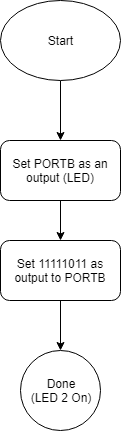
\includegraphics[scale=1]{img/Task1.png}
\end{center}
\newpage
\section{Task 2 - Pulse Width Modulation (PWM)}
\textit{Modify the program in Task 1 to obtain Pulse Width Modulation (PWM). The frequency should be
fixed, but the duty cycle should be possible to change. Use two push buttons to change the duty
cycle up and down. Use interrupt for each pushbutton. The duty cycle should be possible to
change from 0 percent up to 100 percent in steps of 5 percent. Connect the output to an oscilloscope, to visualize
the change in duty cycle.}

\lstset{style=Asm}
\begin{lstlisting}
;>>>>>>>>>>>>>>>>>>>>>>>>>>>>>>>>>>>>>>>>>>>>>>>>>>>>>>>>>>>
; 1DT301, Computer Technology I
; Date: 2019-10-04
; Author:
; Loic GALLAND
; Leonardo PEDRO
;
; Lab number: 4
; Title: Timer and UART
;
; Hardware: STK600, CPU ATmega2560
;
; Function: Program that creates a Pulse Width Modulation using a timer interrupt. When clicking on buttons it will increase or decrease the amount of time in 1s that the LEDs will be on.
;			When the Duty cycle is 50 percent then the LEDs are 0.5s ON and 0.5s OFF. If the Duty cycle is 20 percent, then the LEDs will be ON for 0.2s and OFF 0.8s.
; 
; Input ports: PORTD to control the switches
;
; Output ports: PORTB for the LEDs 
;
; Subroutines: If applicable.
; Included files: m2560def.inc
;<<<<<<<<<<<<<<<<<<<<<<<<<<<<<<<<<<<<<<<<<<<<<<<<<<<<<<<<<<<
.include "m2560def.inc"

.org 0x00
rjmp restart

.org OVF0addr	;Address of the Timer Interrupt number 0
rjmp timer0_int

.org INT0addr	;Address of the Interrupt number 0
rjmp PLUS

.org INT1addr ;Address of the Interrupt number 1
rjmp MINUS

.org 0x72

restart:;To initialize everything
ldi r16, LOW(RAMEND) ; initialize SP, Stackpointer
out SPL, r16
ldi r16, HIGH(RAMEND)
out SPH, r16

ldi r16, 0xFF	;Set PORTB as output
out DDRB, r16

ldi r16, 0x00	;Set PORTD as input
out DDRD, r16

ldi r18, 0b11111111	;Initialize LED state
out portb,r18

ldi r20,0b00001010 ;Setting INT0-INT1 into falling edge
sts EICRA,r20
ldi r20,0b0000011 ;Enable INT0-INT1
out EIMSK,r20

ldi r16, 0x05 ; prescaler value to TCCR0
out TCCR0B, r16 ; CS2 - CS2 = 101, osc.clock / 1024
ldi r16, 0b00000001; Timer 0 enable flag, TOIE0
sts TIMSK0, r16 ; to register TIMSK
ldi r16, 205 ; starting value for counter. Will count from 205 to 255 and therefore will take 50ms
out TCNT0, r16 ; counter register
sei ; enable global interrupt

.DEF COUNTER = r21	;Counter to counts how many times the program went into the timer interrupt
ldi COUNTER, 0
.DEF Duty = r22	;Register to change the duty cycle 
ldi Duty,10
sei	;Global interrupt enable

start:
nop	;Infinite loop that does nothing so that the timer interrupt can interruot something
rjmp start

timer0_int:	;Timer interrupt
	push r16	;Push to Stack and input to SREG, so that no other interrupt interrupts the timer interrupt
	in r16, SREG ;	
	push r16	;
	

	ldi r16, 205 ; starting value for counter.
	out TCNT0, r16
	inc COUNTER	;Increase by 1 the COUNTER

	cpi COUNTER, 20	;Checks if the COUNTER = 20
	Breq reset	;If it is, then reset
	
	cp COUNTER, Duty	;As long as the COUNTER is less than the Duty then turn ON the LEDS.
	BRLT ON				;Otherwise turn OFF the LEDs
	
	OFF:	;Routine for turning off the LEDs
		ldi r18,0xFF
		out PortB,r18
	rjmp END	;Jumps to END routine so that does not go into the ON and reset routine.

	ON:		;Rountine for turning ON the LEDs
		ldi r18,0x00
		out PORTB,r18
	rjmp END	;Jumps to END routine so that does not go into the reset routine.

	reset: 
		ldi COUNTER,0	;Reset the COUNTER
	END:	
		pop r16 ; restore SREG
		out SREG, r16	;Enables the interrupts again. 
		pop r16 ; restore register
reti	;Return from timer interrupt

PLUS:	;Interrupt to increase the Duty cycle
cpi Duty,20	;Checks if duty =20. Do nothing if it is because 20 should be the maximum.
breq DONE2
inc Duty	;Otherwise increase the Duty by 1

DONE2: nop	;Do nothing

RETI	;return from interrupt

MINUS:	;Interrupt to decrease the Duty Cycle 
cpi Duty,0	;Checks if duty =0. Do nothing if it is because 0 should be the minimum.
breq DONE

dec Duty	;Decrease Duty by 1

DONE: nop	;Do nothing
RETI	;return from interrupt
\end{lstlisting}
\newpage
This is the flowchart of the task 2:
\begin{center}
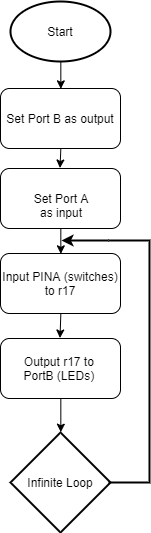
\includegraphics[scale=0.8]{img/Task2.png}
\end{center}

\newpage
\section{Task 3 -Serial communication}
\textit{Write a program in Assembly that uses the serial communication port0 (RS232). Connect a
computer to the serial port and use a terminal emulation program. (Ex. Hyper Terminal)
The program should receive characters that are sent from the computer, and show the code on
the LEDs.}

\lstset{style=Asm}
\begin{lstlisting}
;>>>>>>>>>>>>>>>>>>>>>>>>>>>>>>>>>>>>>>>>>>>>>>>>>>>>>>>>>>>
; 1DT301, Computer Technology I
; Date: 2019-10-04
; Author:
; Loic GALLAND
; Leonardo PEDRO
;
; Lab number: 4
; Title: Timer and UART
;
; Hardware: STK600, CPU ATmega2560
;
; Function: Program that when we type a letter to the terminal it will show the ascii binary code of that letter to the LEDs. Using UART.
; 
; Input ports: Port0 (RS232) VGA 
;
; Output ports: PORTB for the LEDs 
;
; Subroutines: If applicable.
; Included files: m2560def.inc
; The code for this exercice was taken from the lecture.
;<<<<<<<<<<<<<<<<<<<<<<<<<<<<<<<<<<<<<<<<<<<<<<<<<<<<<<<<<<<
.include "m2560def.inc"

.org 0x00
rjmp start

.org 0x72

start:	;To initialize everything
	ldi r16,0xFF	;PORTB outputs
	out DDRB, r16
	
	out PORTB,r16	;Iniatial value to outputs

	ldi r16, 12	;osc = 1MHz, 4800 bps => UBBRR = 12
	sts UBRR1L , r16	;Store Prescaler value in UBRR1L

	ldi r16, (1<<RXEN1)	;Set RX enable flags 
	sts UCSR1B, r16

GetChar:	;Receive data
	lds r16, UCSR1A	;read UCSR1A I/0 register to r16
	sbrs r16,RXC1	;RXC1=1 -> new Character
	rjmp GetChar	;RXC1=0 -> no character received
	lds r18,UDR1	;Read character in UDR

Port_output:	;Show data on the LEDs
	com r18	;COM to have the 1s become 0s as asked for the exercice
	out PORTB,r18	;Write character to PORTB 
	com r18	;COM again to make it normal 
\end{lstlisting}

This is the flowchart of the task 3:
\begin{center}
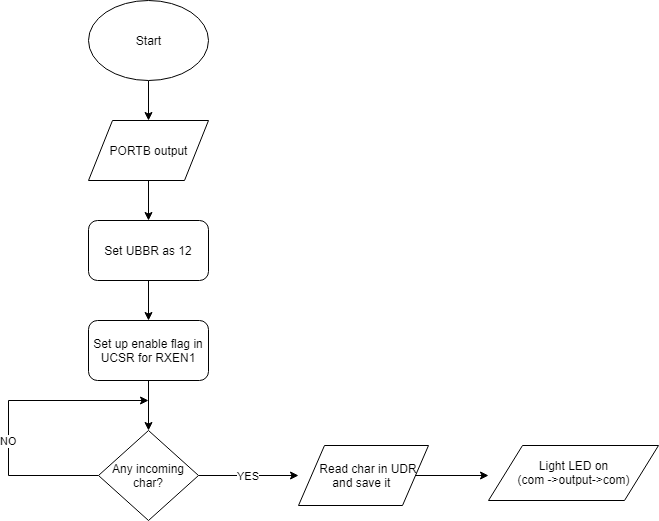
\includegraphics[scale=0.7]{img/TASK3.png}
\end{center}
\newpage
\section{Task 4 - Serial communication with echo}
\textit{Modify the program in task 3 to obtain an echo, which means that the received character should
also be sent back to the terminal. This could be used as a confirmation in the terminal, to ensure
that the character has been transferred correctly.}

\lstset{style=Asm}
\begin{lstlisting}
;>>>>>>>>>>>>>>>>>>>>>>>>>>>>>>>>>>>>>>>>>>>>>>>>>>>>>>>>>>>
; 1DT301, Computer Technology I
; Date: 2019-10-04
; Author:
; Loic GALLAND
; Leonardo PEDRO
;
; Lab number: 4
; Title: Timer and UART
;
; Hardware: STK600, CPU ATmega2560
;
; Function: Program that when we type a letter to the terminal it will show the ascii binary code of that letter to the LEDs.
;			And then sends the letter back to the terminal. Using UART
; Input ports: Port0 (RS232) VGA 
;
; Output ports: PORTB for the LEDs 
;
; Subroutines: If applicable.
; Included files: m2560def.inc
; The code for this exercice was taken from the lecture.
;<<<<<<<<<<<<<<<<<<<<<<<<<<<<<<<<<<<<<<<<<<<<<<<<<<<<<<<<<<<
.include "m2560def.inc"

.org 0x00
rjmp start

.org 0x72

start:
	ldi r16,0xFF	;Set PORTB as output
	out DDRB, r16
	
	out PORTB,r16	;Iniatialize LEDs state

	ldi r16, 12		;osc = 1MHz, 4800 bps => UBBRR = 12
	sts UBRR1L , r16	;Store Prescaler value in UBRR1L

	ldi r16, (1<<RXEN1 | 1<<TXEN1);Set RX and TX enable flags 
	sts UCSR1B, r16

GetChar:	;Receive data
	lds r16, UCSR1A	;read UCSR1A I/0 register to r16
	sbrs r16,RXC1	;RXC1=1 -> new Character
	rjmp GetChar	;RXC1=0 -> no character received
	lds r18,UDR1	;Read character in UDR

Port_output:	;Show Data on LEDs
	com r18
	out PORTB,r18	;Write character to PORTB 
	com r18

PutChar:	;Show data back to the terminal
	lds r16, UCSR1A	;Read UCSR1A i/O register to r16
	sbrs r16, UDRE1	;UDRE1 =1 => buffer is empty 
	rjmp PutChar	;UDRE1 = 0 => buffer is not empty
	sts UDR1,r18	;write character to UDR1
	rjmp GetChar	;Return to loop
\end{lstlisting}

%\newpage
This is the flowchart of the task 4:
\begin{center}
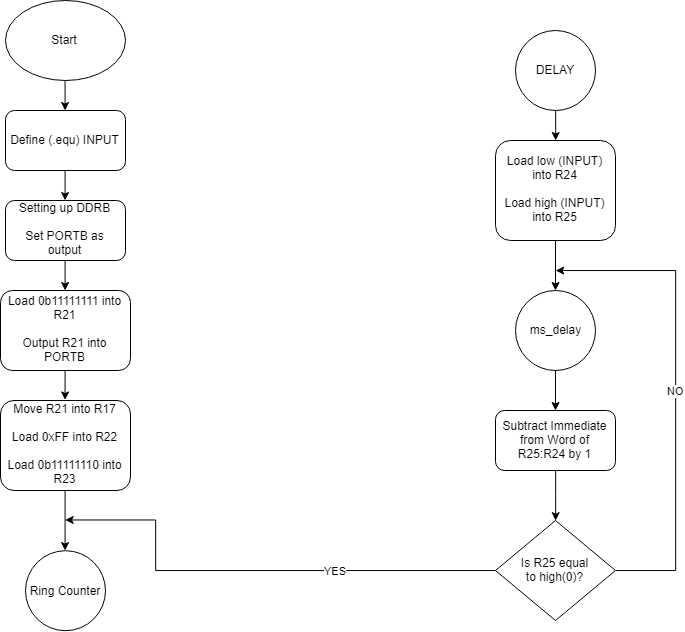
\includegraphics[scale=0.7]{img/Task4.png}
\end{center}
\newpage
\section{Task 5 - Serial communication using Interrupt}
\textit{Do task 3 and 4, but use Interrupt instead of polled UART.
(USART, Rx Complete, USART Data Register Empty and
USART, Tx Complete)}

\lstset{style=Asm}
\begin{lstlisting}
;>>>>>>>>>>>>>>>>>>>>>>>>>>>>>>>>>>>>>>>>>>>>>>>>>>>>>>>>>>>
; 1DT301, Computer Technology I
; Date: 2019-10-04
; Author:
; Loic GALLAND
; Leonardo PEDRO
;
; Lab number: 4
; Title: Timer and UART
;
; Hardware: STK600, CPU ATmega2560
;
; Function: Program that when we type a letter to the terminal it will show the ascii binary code of that letter to the LEDs.
;			And then sends the letter back to the terminal. Using USART Interrupt
;
; Input ports: Port0 (RS232) VGA 
;
; Output ports: PORTB for the LEDs 
;
; Subroutines: If applicable.
; Included files: m2560def.inc
; The code for this exercice was taken from the lecture.
;<<<<<<<<<<<<<<<<<<<<<<<<<<<<<<<<<<<<<<<<<<<<<<<<<<<<<<<<<<<
.include "m2560def.inc"

.org 0x00
rjmp start

.org URXC1addr	;USART Interrupt
rjmp GetChar

.org 0x72

start:
	ldi r16,LOW(RAMEND)	;iniatilize SP
	out SPL,r16
	ldi r16,HIGH(RAMEND)
	out SPH,r16

	ldi r16,0xFF	;Set PORTB as output
	out DDRB, r16
	out PORTB,r16	;Initialize LEDs

	ldi r16, 12		;osc = 1MHz, 4800 bps => UBBRR = 12
	sts UBRR1L , r16	;Store Prescaler value in UBRR1L

	ldi r16, 0b10011000;Set RX, TX enable flags and RXCIE = 1
	sts UCSR1B, r16
	sei	;Set global interrupt flag

Main_loop:
nop		;Infinite loop that does nothing
rjmp Main_loop

GetChar:	;Receive data
	lds r16, UCSR1A	;read UCSR1A I/0 register to r16
	lds r18,UDR1	;Read character in UDR

Port_output:	;Show data on the LEDs
	com r18
	out PORTB,r18	;Write character to PORTB 
	com r18

PutChar:	;Sends back the character to the Terminal
	lds r16, UCSR1A	;Read UCSR1A i/O register to r16
	sts UDR1,r18	;write character to UDR1
RETI	;Return from interrupt
\end{lstlisting}

%\newpage
This is the flowchart of the task 5:
\begin{center}
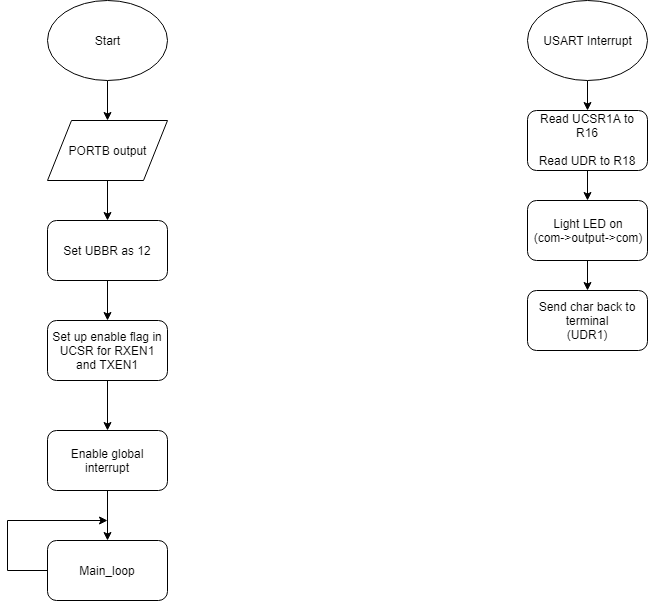
\includegraphics[scale=0.7]{img/Task5.png}
\end{center}

% Prints your bibliography database xxx.bib
\bibliographystyle{IEEEtran}
\bibliography{ref.bib}

\end{document}
